\documentclass[10pt]{article}
\usepackage[a4paper,margin=0.65in]{geometry}
\usepackage{amsmath,amssymb,graphicx,booktabs,multirow,array,float,tabularx}
\usepackage[table]{xcolor}
\usepackage{capt-of,hyperref,fvextra}
\DeclareMathSizes{8}{8}{6}{5}
\DeclareMathSizes{8.5}{9}{6}{5}
\definecolor{valfill}{RGB}{231,239,249}
\definecolor{testfill}{RGB}{224,239,234}
\definecolor{basefill}{RGB}{248,249,251}
\definecolor{conffill}{RGB}{255,247,231}
\definecolor{learnfill}{RGB}{235,246,240}
\definecolor{valink}{RGB}{38,83,123}
\definecolor{testink}{RGB}{34,93,82}
\definecolor{confink}{RGB}{142,91,24}
\definecolor{learnink}{RGB}{30,99,78}
\definecolor{upgreen}{RGB}{24,115,62}
\definecolor{downred}{RGB}{169,48,46}
\definecolor{samegray}{RGB}{95,102,112}
\newcommand{\upchg}[1]{\,\textcolor{upgreen}{(\ensuremath{\uparrow#1})}}
\newcommand{\downchg}[1]{\,\textcolor{downred}{(\ensuremath{\downarrow#1})}}
\newcommand{\callup}[1]{\,\textcolor{downred}{(\ensuremath{\uparrow#1})}}
\newcommand{\calldown}[1]{\,\textcolor{upgreen}{(\ensuremath{\downarrow#1})}}
\newcommand{\samechg}[1]{\,\textcolor{samegray}{(=#1)}}

\hypersetup{hidelinks,pdfauthor={Sihang Cai, Rongjunchen Zhang, Wenxu Jia, Yipu Gong, Tao Jin}}
\setlength{\emergencystretch}{2em}
\title{When Should a Vision Specialist Defer?\\\large Supplementary Material: Learned Routing}
\date{}
\begin{document}
\maketitle
\section{Experimental Scope and Naming}
Learned Routing (LR) denotes the shared pre-call input and routing framework. The four-state instantiation is $\mathrm{LR}_{4S}$; $\mathrm{LR}_{PH}$ adapts the post-hoc deferral loss~\cite{posthocdefer} to the same backbone and visible features. The main experiment uses normalized $\mathrm{LR}_{4S}$, abbreviated LR. These names distinguish our implementations, not newly invented versions of the underlying deferral loss.

The main experiment and Table 3 use different training settings. The main experiment uses 80 newly fitted router heads with full-budget validation selection. The training-objective and scoring comparison uses the earlier 0--25\% checkpoint-selection rule for all trained variants. Its four four-state score rows share identical weights. We do not interpret its comparison with post-hoc deferral as a comparison with the final main results under identical training settings. Test sets have been inspected during method development, so this is an exploratory revision rather than an independent blind confirmation.

\section{Data Preparation and Evaluation}
\label{sec:datasets}
Table~\ref{tab:data} lists the examples actually used in this study. The 4 datasets span detection-related localization and event recognition, together with classification and visual reasoning. They are not 4 object-detection benchmarks, and their task scores have different meanings.

\begin{table}[H]
\centering
\caption{Experimental splits. Counts refer to task examples, not uniformly to distinct images. Training denotes the router's full available training split; specialist training provenance is listed separately. Totals are the sums of the three columns after the recorded exclusions.}
\label{tab:data}
\small\setlength{\tabcolsep}{5pt}
\begin{tabular}{@{}llrrrrl@{}}
\toprule
Dataset & Example unit & Train & Validation & Test & Total & Evaluation \\
\midrule
CUB-200-2011 & One image & 4,792 & 1,200 & 5,794 & 11,786 & Top-1 accuracy \\
gRefCOCO & Image--expression pair & 209,344 & 14,229 & 35,263 & 258,836 & Strict localization accuracy \\
NLVR2 & Two images and a statement & 85,042 & 6,982 & 13,937 & 105,961 & Binary accuracy \\
ConstructionSite10k & One image, 4 event labels & 6,308 & 701 & 3,004 & 10,013 & Event macro-F1 \\
\bottomrule
\end{tabular}
\end{table}

\textbf{CUB-200-2011}~\cite{cub} tests fine-grained recognition among 200 bird species, where differences in plumage, shape and local appearance distinguish related categories. We report top-1 class accuracy. The router reserves 1,200 images from the official training partition for validation and excludes two training images identified as near-duplicates of test images, leaving 4,792 training examples. The official 5,794-image test partition is retained.

\textbf{gRefCOCO}~\cite{gref} tests generalized referring-expression localization, including expressions with one, multiple or no matching objects. TestA and testB contribute 19,200 and 16,063 expressions. Our fixed box-based evaluation requires a valid empty answer for no-target examples. Boxes from either model are first filtered at score $\geq0.7$. For target-present examples, greedy one-to-one matching uses generalized intersection over union of at least 0.5; an example is correct only when instance F1 equals one, with no missed or extra instances. This strict correctness measure is distinct from the dataset's official segmentation evaluation and from detection average precision.

\textbf{NLVR2}~\cite{nlvr2} tests whether a natural-language statement is true of an ordered pair of natural images, including counting, attributes and relations across the pair. We report binary accuracy. The prepared training set contains 85,042 usable examples after filtering the source training partition; validation has 6,982, and the two test portions have 6,967 and 6,970. Routing acts on the complete two-image example.

\textbf{ConstructionSite10k}~\cite{construction} contains construction scenes with structured safety annotations. We evaluate 4 event-presence categories: personal-protection, fall-protection, unprotected-edge and excavator-proximity violations. The original 7,009 training images are split into 6,308 for training and 701 for validation; all 3,004 test images are retained. The dataset name is approximate: the prepared partitions contain 10,013 images. We report
\begin{equation}
M_{\rm event}=\frac14\sum_{j=1}^4
\frac{2\mathrm{TP}_j}{2\mathrm{TP}_j+\mathrm{FP}_j+\mathrm{FN}_j},
\label{eq:f1}
\end{equation}
with zero for a class whose denominator is zero. Delegation replaces all 4 event predictions for an image; confusion counts are then recomputed. This is event recognition, not bounding-box average precision.


\clearpage
\subsection{Examples from the 4 Datasets}
\begin{figure}[H]\centering

\includegraphics[width=\textwidth]{figures/dataset_examples.pdf}
\caption{Real validation examples and their recorded annotations. CUB and ConstructionSite use one image, NLVR2 uses an ordered image pair, and gRefCOCO couples an image with an expression. The first record in each validation manifest was selected before viewing the images. Images illustrate the tasks rather than model performance.}
\end{figure}
The gRefCOCO example refers to two separate targets, illustrating why all matching objects must be found. The NLVR2 label evaluates the full statement about the ordered pair. For ConstructionSite, an all-negative image still requires evaluating all 4 event categories. The sample identifiers and original annotations are provided with the figure data.


\section{Full-Budget Training and Threshold Selection}
The specialist and 8.07M-parameter distilled image/text backbone are frozen. Image features, task text where present, hidden states at 90\% specialist depth, prediction summaries and confidence enter separate 128-dimensional projections and layer normalization. Their concatenation feeds a 128-hidden-unit GELU MLP. Training uses paired cross-entropy, uniform sampling, AdamW at 0.003, weight decay 0.01, batch size 256, at most 50 epochs and patience 8. Seeds are 2026--2030. Training inputs alone determine feature standardization.

With paired state probabilities $p_R,p_H,p_B$, the score is
\[
s_\alpha=\frac{p_R-p_H}{(p_R+p_H+2p_B+10^{-8})^\alpha},\qquad
\alpha\in\{0,0.25,0.5,0.75,1\}.
\]
For every epoch and candidate $\alpha$, we sort validation inputs and evaluate exactly $\lfloor kn/100\rfloor$ calls, $k=0,\ldots,100$, retaining original order at ties. Trapezoidal area over actual call fraction selects the epoch and $\alpha$. A tie within an epoch favors smaller $\alpha$; an epoch tie retains the earlier checkpoint. Early stopping uses this criterion. Cross-entropy itself is unchanged. Historical runs saved only their selected checkpoints, so changing checkpoint selection required refitting the 80 heads.

After weights and $\alpha$ are fixed, a separate validation search selects one threshold. At each interior budget, the threshold is the score of the last allowed input. All threshold ties are included only if they fit the quota; otherwise all equal-score ties are excluded. The highest validation metric wins; ties favor fewer calls, then a smaller budget. Budgets 0 and 100\% explicitly mean never and always call. Confidence uses the same endpoint-inclusive search. Test labels do not select weights, normalization or thresholds. Actual test call rates can differ after a threshold is transferred.

\begin{table}[H]
\centering
\caption{Selected normalization strength $\alpha$ for the main experiment, separately chosen on validation data for each pair and seed. M: MiniCPM. Q: Qwen. Across 80 runs, $0,0.25,0.5,0.75,1$ are selected 29, 8, 9, 9 and 25 times. These choices do not describe the earlier Table 3 checkpoints.}
\label{tab:alpha}
\small
\begin{tabular}{lllrrrrr}
\toprule
Task & Specialist & VLM & 2026 & 2027 & 2028 & 2029 & 2030 \\
\midrule
CUB & ResNet-50 & M & 0 & 0 & 0.25 & 0 & 0 \\
CUB & ResNet-50 & Q & 0 & 0 & 0 & 0 & 0.25 \\
CUB & GLSim & M & 0.5 & 0.25 & 0.5 & 0.5 & 0.5 \\
CUB & GLSim & Q & 0 & 0 & 0 & 0 & 0 \\
gRefCOCO & GroundingDINO & M & 0 & 0 & 0 & 0 & 0 \\
gRefCOCO & GroundingDINO & Q & 0 & 0 & 0 & 0 & 0 \\
gRefCOCO & InstanceVG & M & 0.75 & 0.75 & 0.75 & 0.75 & 0.75 \\
gRefCOCO & InstanceVG & Q & 1 & 1 & 1 & 1 & 1 \\
NLVR2 & BEiT3 & M & 1 & 1 & 1 & 1 & 1 \\
NLVR2 & BEiT3 & Q & 1 & 1 & 1 & 1 & 1 \\
NLVR2 & ViLT & M & 1 & 1 & 1 & 1 & 1 \\
NLVR2 & ViLT & Q & 1 & 1 & 1 & 1 & 1 \\
Construction & YOLO26X & M & 0.5 & 0.5 & 0.75 & 0.75 & 0.5 \\
Construction & YOLO26X & Q & 0.75 & 0.5 & 0.25 & 0.25 & 0.75 \\
Construction & RT-DETR-X & M & 0 & 0 & 0.25 & 0 & 0 \\
Construction & RT-DETR-X & Q & 0 & 0.25 & 0.25 & 0 & 0.5 \\
\bottomrule
\end{tabular}
\end{table}


\section{Main Results and Full Curves}
Table~\ref{tab:full} includes both splits. Numerical per-seed cutoffs, comparison operators, chosen epochs and normalization strengths are stored with the revision data. Higher routed performance and fewer calls are different objectives; selected points need not dominate a baseline on both. Zero- and full-call endpoints agree with direct standalone evaluation.
\begin{table}[H]
\centering
\caption{LR results are means over five router seeds (2026--2030); the supplement reports standard deviations. Complete four-way comparison. Scores and actual call rates are percentages. Thresholds selected on the 0--100\% validation grid transfer unchanged to test. Parentheses give LR-minus-confidence differences in percentage points before rounding. Green marks improvement and red degradation: higher scores and fewer calls are better. Bold marks the higher routed score; $\dagger$ exceeds both test endpoints. M: MiniCPM-V-4.5; Q: Qwen3.8-27B-FP8.}
\label{tab:full}
\fontsize{7}{8.4}\selectfont
\setlength{\tabcolsep}{1.2pt}
\renewcommand{\arraystretch}{1.12}
\resizebox{\textwidth}{!}{%
\begin{tabular}{@{}lll>{\columncolor{basefill}}r>{\columncolor{basefill}}r>{\columncolor{conffill}}r>{\columncolor{conffill}}r>{\columncolor{learnfill}}r>{\columncolor{learnfill}}r>{\columncolor{basefill}}r>{\columncolor{basefill}}r>{\columncolor{conffill}}r>{\columncolor{conffill}}r>{\columncolor{learnfill}}r>{\columncolor{learnfill}}r@{}}
\toprule
\multirow{2}{*}{Task} & \multirow{2}{*}{Specialist} & \multirow{2}{*}{VLM} & \multicolumn{6}{c}{\cellcolor{valfill}\textcolor{valink}{Validation}} & \multicolumn{6}{c}{\cellcolor{testfill}\textcolor{testink}{Test}} \\ \cmidrule(lr){4-9}\cmidrule(l){10-15} & & & \textcolor{testink}{spec.} & \textcolor{testink}{vlm.} & \textcolor{confink}{conf.} & \textcolor{confink}{call$_{\rm conf}$} & \textcolor{learnink}{LR$\uparrow$} & \textcolor{learnink}{call$_{\rm LR}\downarrow$} & \textcolor{testink}{spec.} & \textcolor{testink}{vlm.} & \textcolor{confink}{conf.} & \textcolor{confink}{call$_{\rm conf}$} & \textcolor{learnink}{LR$\uparrow$} & \textcolor{learnink}{call$_{\rm LR}\downarrow$} \\
\midrule
CUB-200-2011 & ResNet & M & 98.58 & 27.75 & 98.58 & 0.00 & \textbf{98.62}\upchg{0.03} & 0.40\callup{0.40} & 81.43 & 26.56 & 81.43 & 0.00 & \textbf{81.43}\samechg{0.00} & 0.59\callup{0.59} \\
 & ResNet & Q & 98.58 & 55.08 & 98.58 & 0.00 & \textbf{98.58}\samechg{0.00} & 0.00\samechg{0.00} & 81.43 & 54.82 & 81.43 & 0.00 & \textbf{81.43}\samechg{0.00} & 0.00\samechg{0.00} \\
 & GLSim & M & 98.92 & 27.75 & 98.92 & 0.00 & \textbf{98.95}\upchg{0.03} & 0.40\callup{0.40} & 90.16 & 26.56 & \textbf{90.16} & 0.00 & 90.13\downchg{0.03} & 0.85\callup{0.85} \\
 & GLSim & Q & 98.92 & 55.08 & \textbf{98.92} & 0.00 & 98.92\samechg{0.00} & 0.00\samechg{0.00} & 90.16 & 54.82 & 90.16 & 0.00 & \textbf{90.16}\samechg{0.00} & 0.00\samechg{0.00} \\
\midrule
gRefCOCO & GroundingDINO & M & 56.05 & 64.12 & 64.12 & 100.00 & \textbf{65.91}\upchg{1.79} & 45.80\calldown{54.20} & 26.69 & 50.01 & 50.01 & 100.00 & \textbf{50.23}$^\dagger$\upchg{0.22} & 58.19\calldown{41.81} \\
 & GroundingDINO & Q & 56.05 & 80.60 & 80.60 & 100.00 & \textbf{81.41}\upchg{0.80} & 77.60\calldown{22.40} & 26.69 & 74.47 & 74.47 & 100.00 & \textbf{75.12}$^\dagger$\upchg{0.65} & 88.47\calldown{11.53} \\
 & InstanceVG & M & 75.03 & 64.12 & \textbf{77.17} & 64.99 & 75.67\downchg{1.50} & 14.40\calldown{50.60} & 66.95 & 50.01 & 61.88 & 52.09 & \textbf{67.91}$^\dagger$\upchg{6.04} & 19.04\calldown{33.06} \\
 & InstanceVG & Q & 75.03 & 80.60 & 82.02 & 71.00 & \textbf{83.38}\upchg{1.36} & 45.60\calldown{25.40} & 66.95 & 74.47 & 72.43 & 68.39 & \textbf{76.24}$^\dagger$\upchg{3.81} & 62.00\calldown{6.38} \\
\midrule
NLVR2 & BEiT3 & M & 79.82 & 89.90 & \textbf{90.05} & 85.88 & 89.99\downchg{0.05} & 91.39\callup{5.51} & 80.00 & 90.74 & 90.77 & 85.80 & \textbf{90.80}$^\dagger$\upchg{0.03} & 91.10\callup{5.30} \\
 & BEiT3 & Q & 79.82 & 90.50 & 90.58 & 85.88 & \textbf{91.09}\upchg{0.51} & 84.19\calldown{1.69} & 80.00 & 90.06 & 90.24 & 85.80 & \textbf{90.60}$^\dagger$\upchg{0.36} & 84.34\calldown{1.46} \\
 & ViLT & M & 75.57 & 89.90 & \textbf{89.97} & 95.99 & 89.93\downchg{0.04} & 98.20\callup{2.21} & 76.42 & 90.74 & 90.64 & 95.93 & \textbf{90.69}\upchg{0.05} & 98.06\callup{2.13} \\
 & ViLT & Q & 75.57 & 90.50 & \textbf{90.59} & 95.99 & 90.50\downchg{0.09} & 99.60\callup{3.61} & 76.42 & 90.06 & 89.96 & 95.93 & \textbf{90.07}$^\dagger$\upchg{0.10} & 99.62\callup{3.69} \\
\midrule
ConstructionSite & YOLO26x & M & 18.25 & 20.67 & 22.64 & 93.87 & \textbf{28.71}\upchg{6.06} & 45.73\calldown{48.13} & 18.13 & 22.36 & 25.23 & 92.54 & \textbf{25.88}$^\dagger$\upchg{0.65} & 45.32\calldown{47.22} \\
 & YOLO26x & Q & 18.25 & 25.45 & 26.43 & 92.87 & \textbf{32.80}\upchg{6.37} & 45.14\calldown{47.73} & 18.13 & 27.00 & 25.97 & 92.21 & \textbf{29.80}$^\dagger$\upchg{3.82} & 44.77\calldown{47.44} \\
 & RT-DETR-X & M & 7.64 & 20.67 & 20.67 & 100.00 & \textbf{21.99}\upchg{1.33} & 77.29\calldown{22.71} & 7.89 & 22.36 & 22.36 & 100.00 & \textbf{22.80}$^\dagger$\upchg{0.44} & 78.44\calldown{21.56} \\
 & RT-DETR-X & Q & 7.64 & 25.45 & 25.45 & 100.00 & \textbf{27.23}\upchg{1.78} & 83.08\calldown{16.92} & 7.89 & 27.00 & \textbf{27.00} & 100.00 & 26.78\downchg{0.22} & 83.57\calldown{16.43} \\
\bottomrule
\end{tabular}}
\end{table}

\begin{table}[H]
\centering
\caption{Confidence cutoffs and mean LR validation budgets across five seeds. Each LR seed uses its own validation cutoff unchanged on test; exact per-seed cutoffs are provided in the accompanying data/per\_seed.csv.}
\label{tab:thresholds}
\fontsize{9}{10.799999999999999}\selectfont
\setlength{\tabcolsep}{4pt}
\renewcommand{\arraystretch}{1.12}
\begin{tabular}{@{}lllrrrr@{}}
\toprule
Task & Specialist & VLM & Conf. budget & Conf. cutoff & LR budget & LR cutoff \\
\midrule
CUB-200-2011 & ResNet & M & 0 & Never & 0.4 & Per seed \\
 & ResNet & Q & 0 & Never & 0.0 & Per seed \\
 & GLSim & M & 0 & Never & 0.4 & Per seed \\
 & GLSim & Q & 0 & Never & 0.0 & Per seed \\
\midrule
gRefCOCO & GroundingDINO & M & 100 & Always & 45.8 & Per seed \\
 & GroundingDINO & Q & 100 & Always & 77.6 & Per seed \\
 & InstanceVG & M & 65 & $\geq-0.987771$ & 14.4 & Per seed \\
 & InstanceVG & Q & 71 & $\geq-0.994979$ & 45.6 & Per seed \\
\midrule
NLVR2 & BEiT3 & M & 86 & $>-0.999739$ & 91.4 & Per seed \\
 & BEiT3 & Q & 86 & $>-0.999739$ & 84.2 & Per seed \\
 & ViLT & M & 96 & $\geq-0.99984$ & 98.2 & Per seed \\
 & ViLT & Q & 96 & $\geq-0.99984$ & 99.6 & Per seed \\
\midrule
ConstructionSite & YOLO26x & M & 94 & $\geq-0.490234$ & 45.8 & Per seed \\
 & YOLO26x & Q & 93 & $\geq-0.453369$ & 45.2 & Per seed \\
 & RT-DETR-X & M & 100 & Always & 77.4 & Per seed \\
 & RT-DETR-X & Q & 100 & Always & 83.2 & Per seed \\
\bottomrule
\end{tabular}
\end{table}

\begin{table}[H]
\centering
\caption{Selected outcome counts and gains are five-seed means; available outcome counts are fixed. Test outcome counts at the LR operating point. BC/BW: both correct/wrong; R/H: rescue/harm. Selected rescues, selected harms, missed rescues and avoided harms are counted separately. Construction counts 12,016 events, with routing over 3,004 images. Metric gains are recomputed; macro-F1 is not an event-count ratio.}
\label{tab:outcomes_full}
\fontsize{8.5}{10.2}\selectfont
\setlength{\tabcolsep}{3pt}
\renewcommand{\arraystretch}{1.12}
\begin{tabular}{@{}lllrrrrrrrrr@{}}
\toprule
Task & Specialist & VLM & BC & R & H & BW & Sel. R & Sel. H & Miss R & Avoid H & Gain (pp) \\
\midrule
CUB-200-2011 & ResNet & M & 1,307 & 232 & 3,411 & 844 & 4.6 & 4.6 & 227.4 & 3,406.4 & +0.000 \\
 & ResNet & Q & 2,811 & 365 & 1,907 & 711 & 0.0 & 0.0 & 365.0 & 1,907.0 & +0.000 \\
 & GLSim & M & 1,433 & 106 & 3,791 & 464 & 1.0 & 2.8 & 105.0 & 3,788.2 & -0.031 \\
 & GLSim & Q & 3,032 & 144 & 2,192 & 426 & 0.0 & 0.0 & 144.0 & 2,192.0 & +0.000 \\
\midrule
gRefCOCO & GroundingDINO & M & 6,911 & 10,723 & 2,500 & 15,129 & 9,475.4 & 1,174.4 & 1,247.6 & 1,325.6 & +23.540 \\
 & GroundingDINO & Q & 7,441 & 18,820 & 1,970 & 7,032 & 18,720.8 & 1,641.6 & 99.2 & 328.4 & +48.434 \\
 & InstanceVG & M & 15,007 & 2,627 & 8,602 & 9,027 & 727.6 & 388.2 & 1,899.4 & 8,213.8 & +0.962 \\
 & InstanceVG & Q & 20,838 & 5,423 & 2,771 & 6,231 & 4,753.6 & 1,476.8 & 669.4 & 1,294.2 & +9.292 \\
\midrule
NLVR2 & BEiT3 & M & 10,421 & 2,225 & 729 & 562 & 2,189.4 & 684.6 & 35.6 & 44.4 & +10.797 \\
 & BEiT3 & Q & 10,305 & 2,247 & 845 & 540 & 2,163.4 & 686.4 & 83.6 & 158.6 & +10.598 \\
 & ViLT & M & 9,940 & 2,706 & 711 & 580 & 2,693.8 & 704.8 & 12.2 & 6.2 & +14.271 \\
 & ViLT & Q & 9,761 & 2,791 & 890 & 495 & 2,788.2 & 886.8 & 2.8 & 3.2 & +13.643 \\
\midrule
ConstructionSite & YOLO26x & M & 8,176 & 1,198 & 2,109 & 533 & 1,139.6 & 803.4 & 58.4 & 1,305.6 & +7.751 \\
 & YOLO26x & Q & 9,508 & 1,282 & 777 & 449 & 1,231.6 & 315.0 & 50.4 & 462.0 & +11.667 \\
 & RT-DETR-X & M & 6,060 & 3,314 & 1,945 & 697 & 3,288.6 & 1,452.4 & 25.4 & 492.6 & +14.912 \\
 & RT-DETR-X & Q & 7,329 & 3,461 & 676 & 550 & 3,448.0 & 574.8 & 13.0 & 101.2 & +18.896 \\
\bottomrule
\end{tabular}
\end{table}

\begin{figure}[p]\centering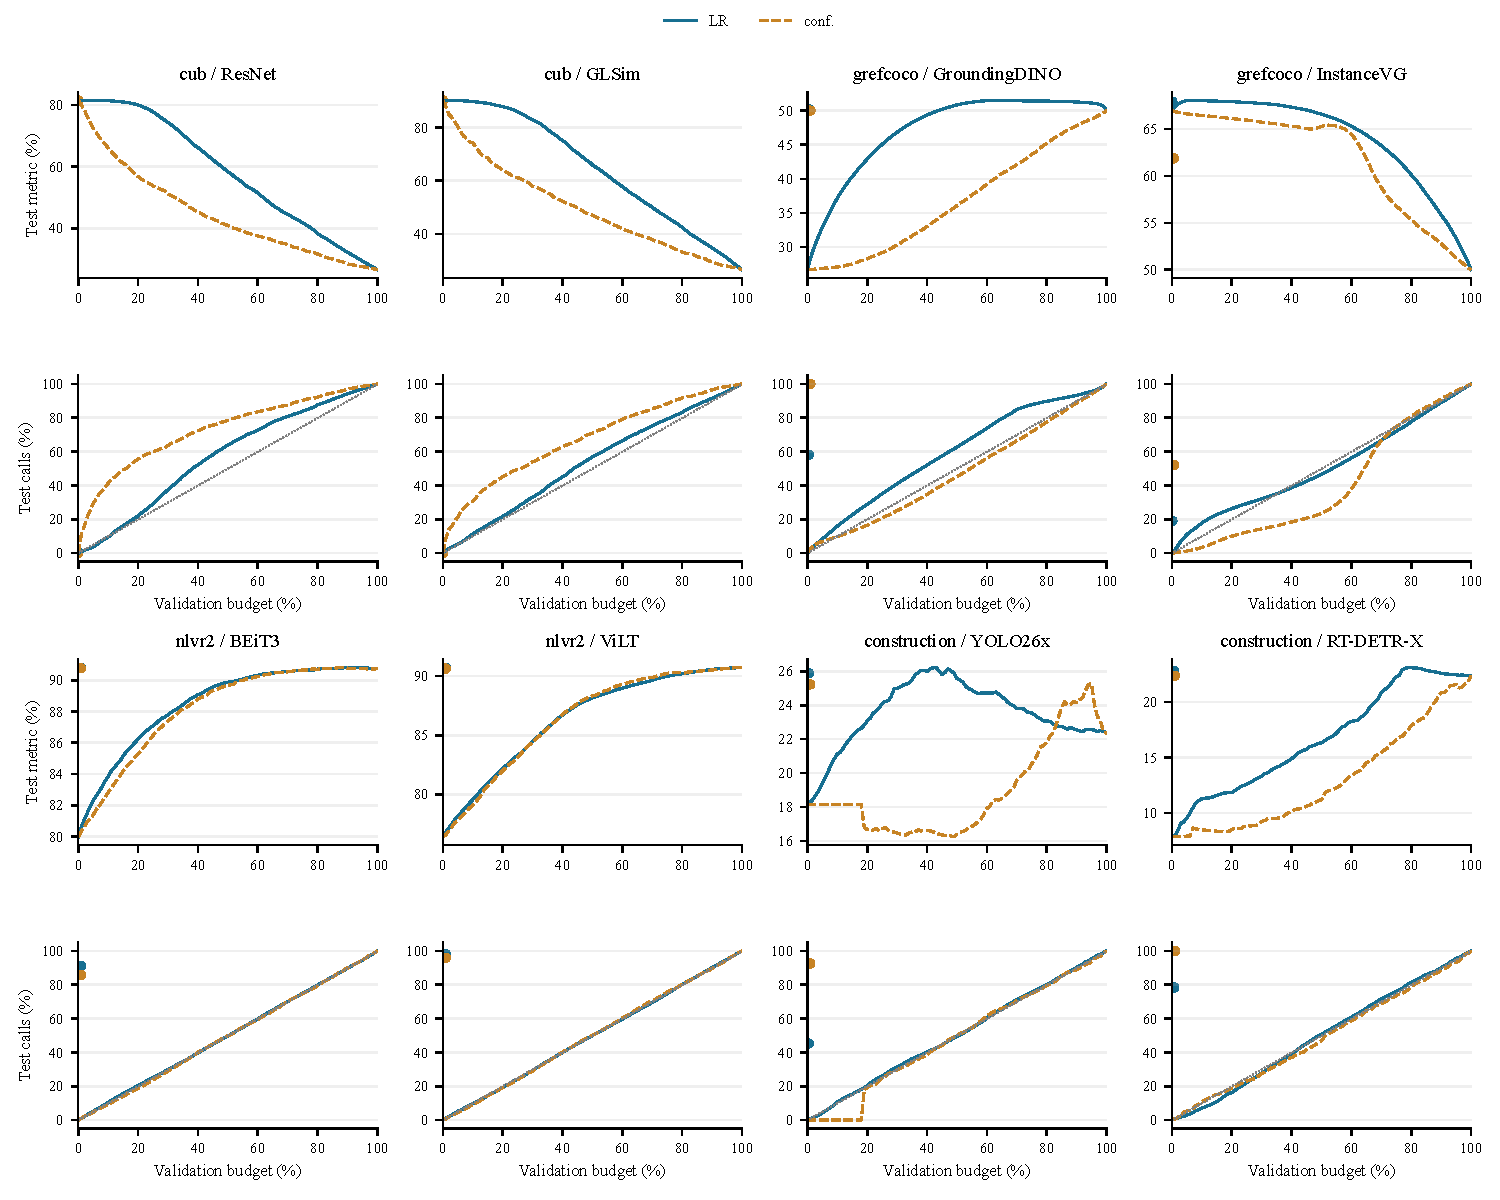
\includegraphics[width=\textwidth]{figures/budget_all_m.pdf}\caption{LR and confidence results for MiniCPM. Horizontal axes show the nominal validation budget; panels report test performance and transferred test call rates, including both endpoints.}\end{figure}
\begin{figure}[p]\centering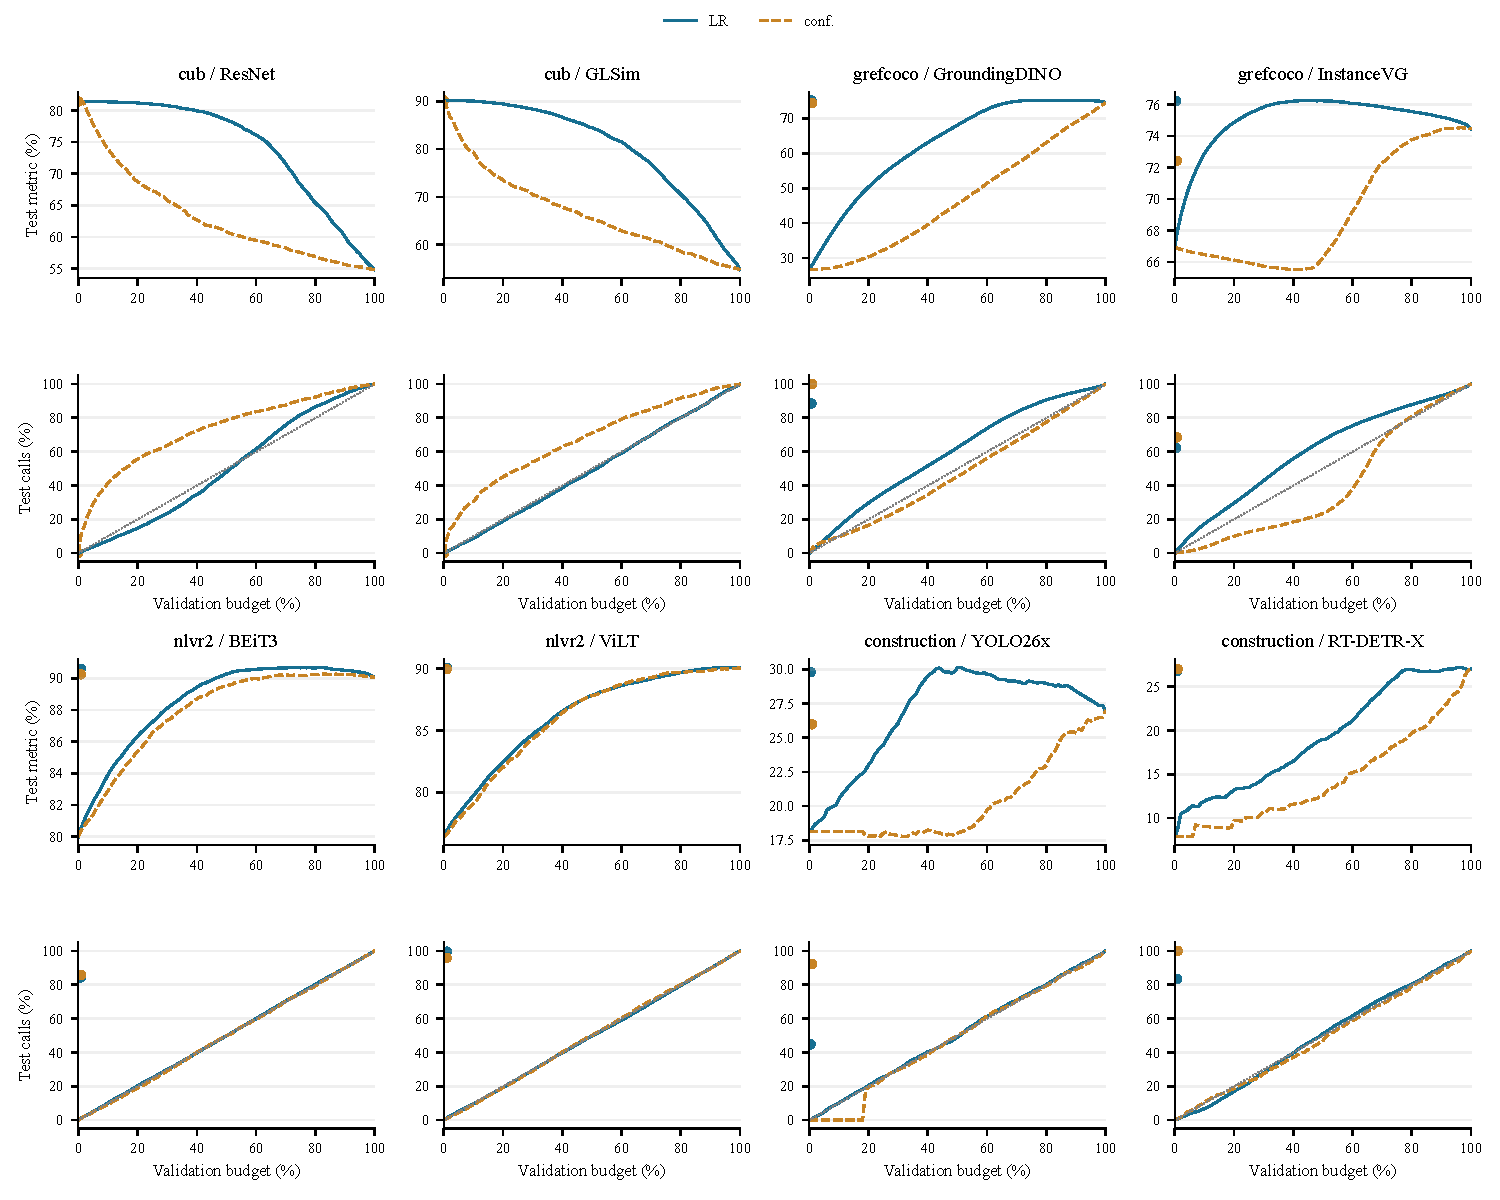
\includegraphics[width=\textwidth]{figures/budget_all_q.pdf}\caption{LR and confidence results for Qwen. Same conventions.}\end{figure}
\clearpage
\begin{figure}[p]\centering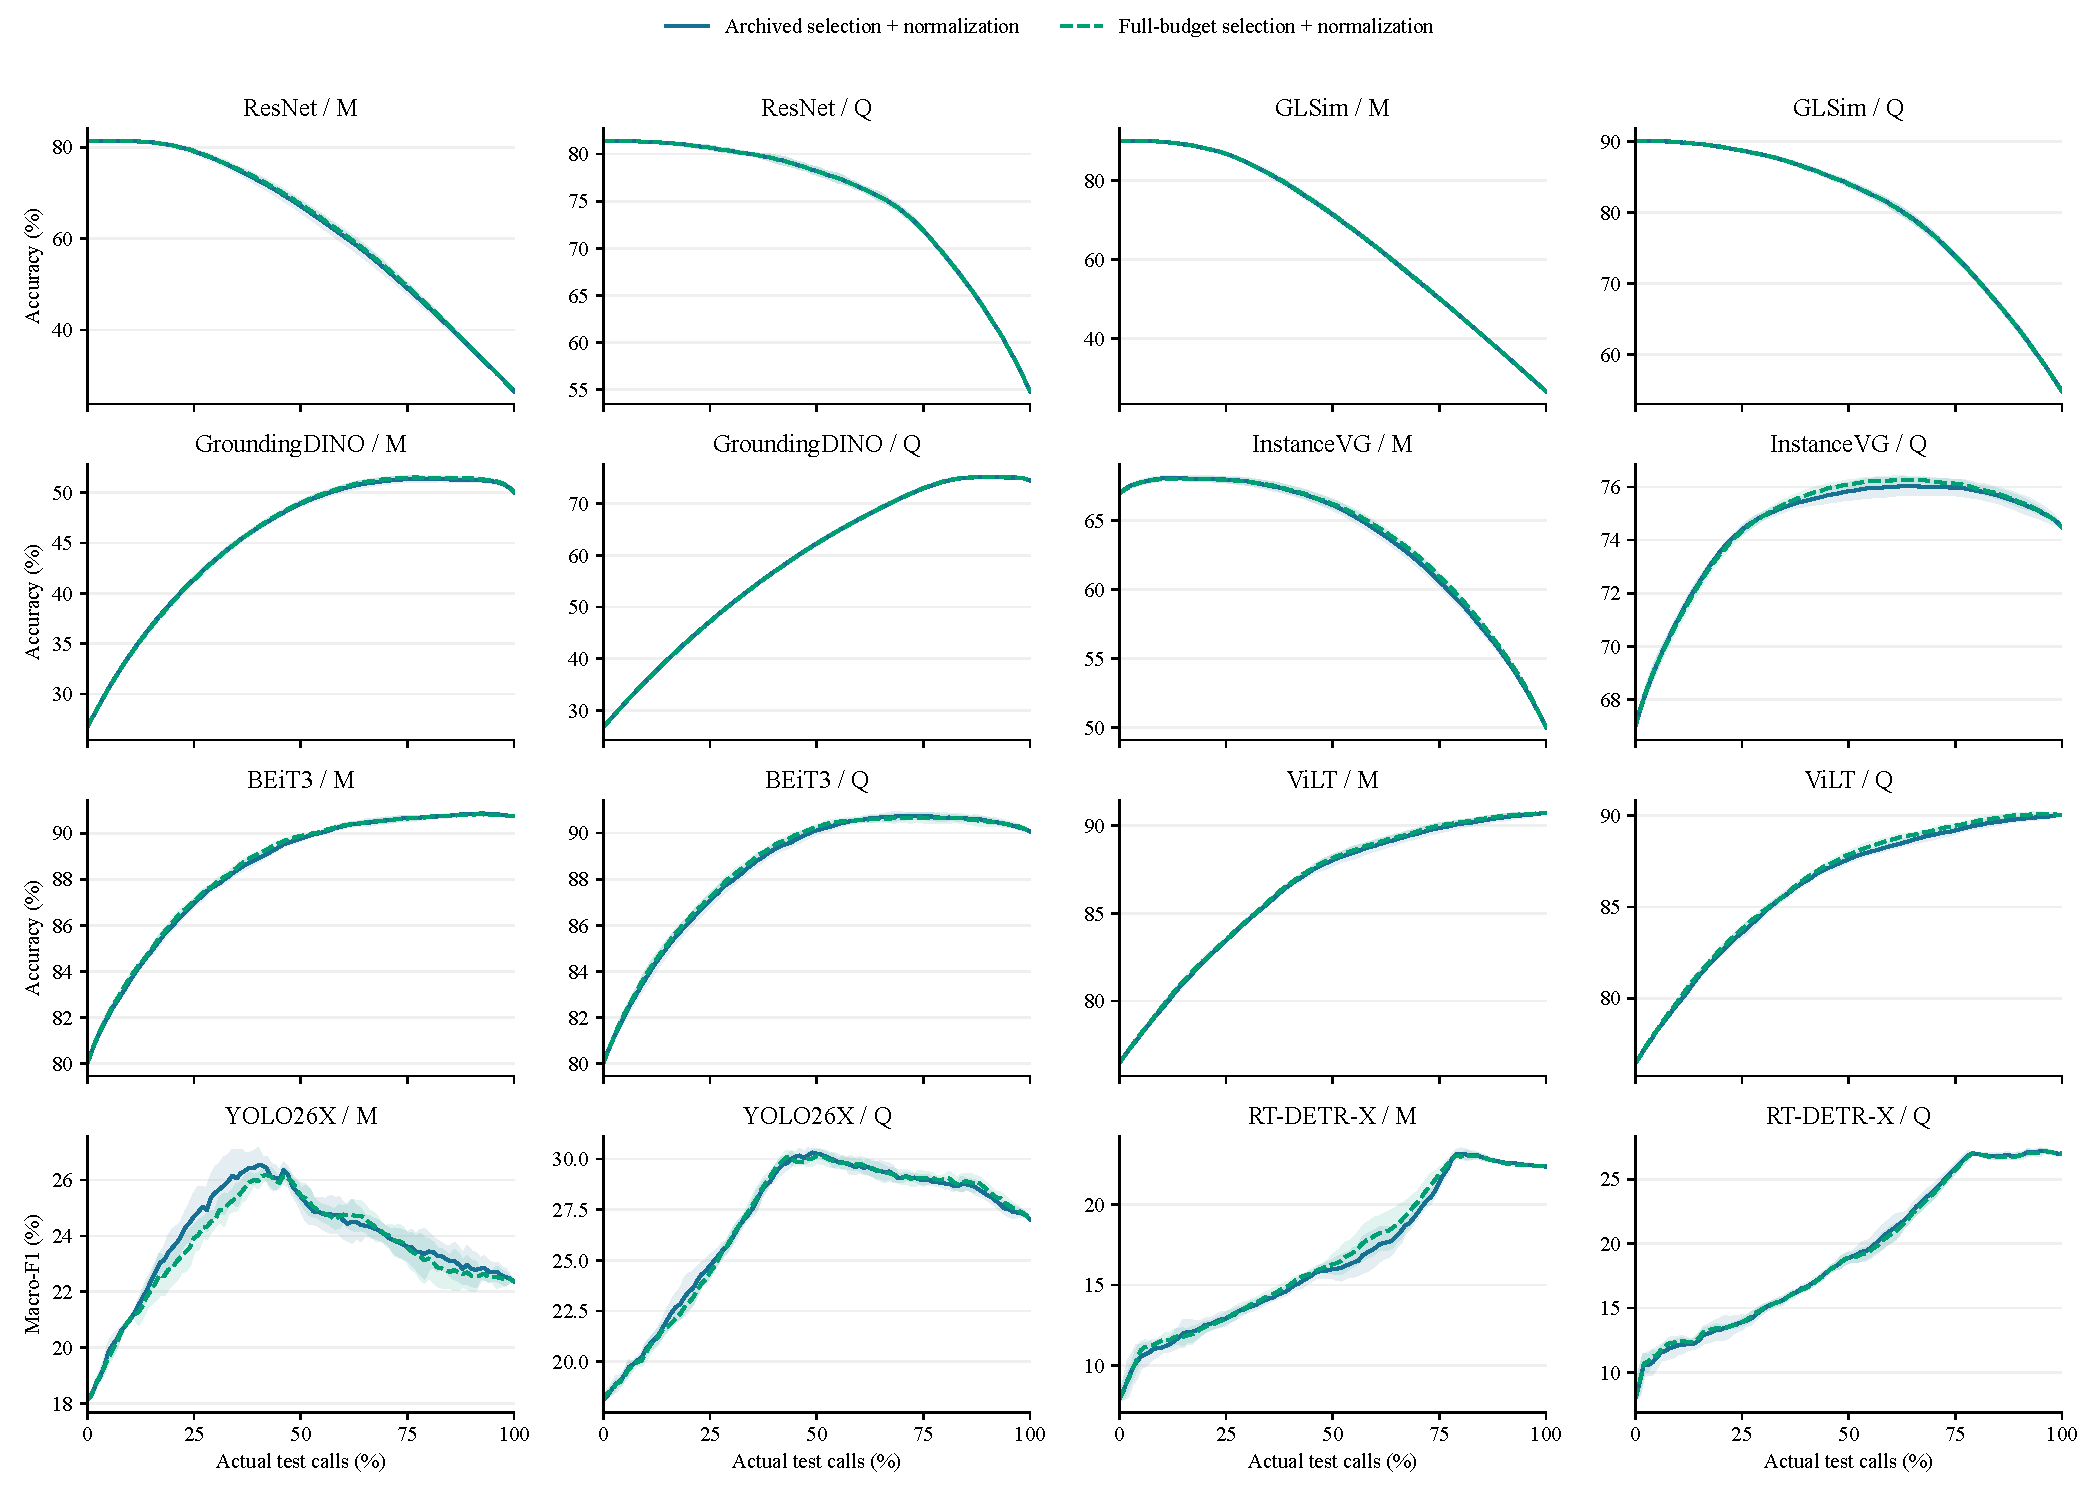
\includegraphics[width=\textwidth]{figures/full_budget_reselection.pdf}\caption{Old checkpoints with normalization versus full-budget checkpoint/normalization selection at identical actual calls. Five-seed means and standard-deviation bands. This isolates the incremental reselection effect after changing the score.}\end{figure}
\clearpage
\section{Training Objectives and Ranking Scores}
This section gives the settings behind Table 3 of the main paper. The table evaluates the full 0--100\% call curve, but the trained heads were selected using the earlier 0--25\% validation criterion. Evaluation range and training selection range are distinct. In contrast, the main table selects weights using the full-budget criterion. Table 3 therefore compares objectives within the earlier experiments; it should not be read as a comparison of every objective under the final main-table training settings.

Four-state, three-state, gain and post-hoc runs use the same inputs, architecture except necessary head dimensions, optimizer settings, seeds and original 0--25\% validation checkpoint-selection range. All four-state score variants share 80 identical checkpoints. Normalization strength alone is chosen by full-budget validation area.

Specialist and VLM answers remain fixed. Other archived post-hoc cost coefficients are not selected using test results. The reported averages are descriptive, not significance tests.
\subsection{Targets, Outputs and All Seven Table Rows}
Let $C=(1,1)$, $R=(0,1)$, $H=(1,0)$ and $B=(0,0)$ denote both-correct, rescue, harm and both-wrong outcomes, respectively, with specialist correctness first. A four-output head produces logits $\ell_k$ and probabilities $p_k=\exp(\ell_k)/\sum_j\exp(\ell_j)$ for $k,j\in\{C,R,H,B\}$. Thus $p_R$ estimates the chance that replacement fixes an error, $p_H$ that it causes an error, and $p_B$ that both answers are wrong. For construction, the target $q_k$ is the fraction of four event labels in state $k$. There is one predicted distribution and one score per image, and a call replaces all four event answers. Every row sorts scores in descending order: larger scores receive calls first.

\paragraph{Row 1: post-hoc deferral, score $r$.}
One unrestricted scalar output $r=f_\theta(\mathcal I)$ replaces the four logits. With $e_S=1-c_S$ and $e_L=1-c_L$, training minimizes the sample mean of
\[
e_S\log(1+\exp(-r))+e_L\log(1+\exp(r)).
\]
For construction, the two errors are averaged over events. A specialist error favors a positive score, and a VLM error a negative score. Added call cost is zero. Ranking uses $r$ directly, without a probability conversion or a fixed zero threshold.

\paragraph{Row 2: three-state classification, score $p_R-p_H$.}
The targets are rescue, harm and unchanged ($U=C\cup B$). Three logits feed a three-way softmax. Training minimizes cross-entropy $-\sum_{k\in\{R,H,U\}}q_k\log p_k$, averaged over examples. Construction again uses event fractions as targets. The score subtracts predicted harm probability from predicted rescue probability. Both unchanged outcomes have zero gain and share one target.

\paragraph{Row 3: gain regression, score $\widehat\Delta$.}
One unrestricted scalar $\widehat\Delta=f_\theta(\mathcal I)$ predicts $d=c_L-c_S$, which is $+1$ for rescue, $-1$ for harm and $0$ for either unchanged outcome. Construction uses $d=\tfrac14\sum_{j=1}^{4}(c_{L,j}-c_{S,j})$. Training minimizes the sample mean of $(\widehat\Delta-d)^2$. The scalar prediction is the ranking score, without softmax, sigmoid or clipping.

\paragraph{Row 4: four-state classification, probability difference.}
The four-state head minimizes cross-entropy $-\sum_{k\in\{C,R,H,B\}}q_k\log p_k$. Its score $p_R-p_H$ estimates expected correctness gain from replacement and lies in $[-1,1]$. Neither unchanged outcome contributes to the difference. Rows 5--7 reuse exactly these head weights and probabilities.

\paragraph{Row 5: four-state classification, rescue-to-harm ratio.}
The score $\log(p_R/p_H)=\ell_R-\ell_H$ measures rescue relative to harm, instead of subtracting probabilities. The implementation subtracts logits, avoiding division by very small probabilities. The unchanged states do not enter the ratio explicitly.

\paragraph{Row 6: four-state classification, error ratio $r_{4S}$.}
The predicted specialist error rate is $p_R+p_B$, and the predicted VLM error rate is $p_H+p_B$. The score is
\[
r_{4S}=\log\frac{p_R+p_B}{p_H+p_B}
=\operatorname{LSE}(\ell_R,\ell_B)-\operatorname{LSE}(\ell_H,\ell_B),
\]
where $\operatorname{LSE}(a,b)=\log(\exp(a)+\exp(b))$ is evaluated by a numerically stable log-sum-exp operation. Both-wrong probability enters both error rates. For positive conditional error rates, setting the derivative of the expected row-1 loss to zero gives $\exp(r)=\mathbb E[e_S\mid\mathcal I]/\mathbb E[e_L\mid\mathcal I]$. Row 6 estimates this ratio from four-state probabilities, while row 1 fits a scalar separately. Their fitted rankings need not coincide.

\paragraph{Row 7: four-state classification, normalized gain $s_\alpha$.}
The score is
\[
s_\alpha=\frac{p_R-p_H}{(p_R+p_H+2p_B+10^{-8})^\alpha}.
\]
The denominator is the sum of the two predicted error rates, with $10^{-8}$ added for numerical stability. At $\alpha=0$, the score equals row 4. Ignoring that constant, at $\alpha=1$ it is $(a-b)/(a+b)$ for $a=p_R+p_B$ and $b=p_H+p_B$, which orders examples like $a/b$ and hence row 6. Intermediate values partially normalize gain. For Table 3, each pair and seed selects $\alpha\in\{0,0.25,0.5,0.75,1\}$ by full-budget validation area with the row-4 checkpoint fixed. This differs from the main experiment's joint epoch and $\alpha$ selection.

\subsection{How the Table Values Are Calculated}
For each variant, model pair and seed, sort the $n$ test examples by score, preserving original order at ties. At budget index $k=0,\ldots,100$, call the VLM on the first $m_k=\lfloor kn/100\rfloor$ examples and retain the specialist elsewhere. Let $b_k=m_k/n$ and $M_k$ be the resulting task metric as a fraction. The full-budget mean in percentage units is
\[
A=100\sum_{k=1}^{100}\frac{M_{k-1}+M_k}{2}(b_k-b_{k-1}).
\]
The interval runs from $b_0=0$ to $b_{100}=1$, so no further range normalization is needed. This is a trapezoidal average of the entire curve, not the best test threshold. For CUB, gRefCOCO and NLVR2, $M_k$ is task accuracy. For construction, the combined predictions determine new true-positive, false-positive and false-negative counts at each budget. Then $M_k$ averages $2\mathrm{TP}/(2\mathrm{TP}+\mathrm{FP}+\mathrm{FN})$ over four events, assigning zero when the denominator is zero.

Each task column averages $A$ over four model pairs and five seeds. For each seed, Avg. averages four pairs within each task and then gives equal weight to the four tasks. The displayed Avg. is the mean of those five seed-level values, and its SD uses divisor $5-1$. The final column subtracts the unrounded post-hoc Avg. from the unrounded variant Avg. and rounds to two decimals. Subtracting displayed rounded means can therefore differ by 0.01 points. No value pools examples across tasks or selects the best seed.

\begin{table}[H]\centering
\captionof{table}{Full-budget means (\%). Avg.: equal-task mean (five-seed SD). $\Delta$: gain over $\mathrm{LR}_{PH}$ (pp). Shared weights for $\mathrm{LR}_{4S}$. Earlier selection settings in supplement. CS: ConstructionSite.}
\label{tab:objective}
\fontsize{8}{9.5}\selectfont
\setlength{\tabcolsep}{1.5pt}
\begin{tabular}{@{}llrrrrrr@{}}
\toprule
Variant & Score & CUB & gRef & NLVR & CS & Avg. & $\Delta$ \\
\midrule
$\mathrm{LR}_{PH}$ & $r$ & 65.86 & 59.37 & 87.33 & 21.24 & 58.45 (0.07) & -- \\
\midrule
3-state & $p_R-p_H$ & 71.27 & 60.13 & 86.34 & 21.77 & 59.88 (0.06) & \textcolor{upgreen}{+1.43} \\
Gain & $\widehat\Delta$ & 71.01 & 59.97 & 86.29 & 21.61 & 59.72 (0.04) & \textcolor{upgreen}{+1.27} \\
\midrule
$\mathrm{LR}_{4S}$ & $p_R-p_H$ & 71.30 & 60.10 & 86.43 & 21.69 & 59.88 (0.06) & \textcolor{upgreen}{+1.43} \\
$\mathrm{LR}_{4S}$ & $\log(p_R/p_H)$ & 67.80 & 59.84 & 87.36 & 21.11 & 59.03 (0.09) & \textcolor{upgreen}{+0.58} \\
$\mathrm{LR}_{4S}$ & $r_{4S}$ & 67.63 & 59.90 & 87.36 & 21.30 & 59.05 (0.10) & \textcolor{upgreen}{+0.60} \\
\rowcolor{learnfill}
$\mathrm{LR}_{4S}$ & $s_\alpha$ & 71.37 & 60.66 & 87.36 & 21.63 & 60.25 (0.06) & \textcolor{upgreen}{+1.81} \\
\bottomrule
\end{tabular}
\end{table}
\begin{figure}[p]\centering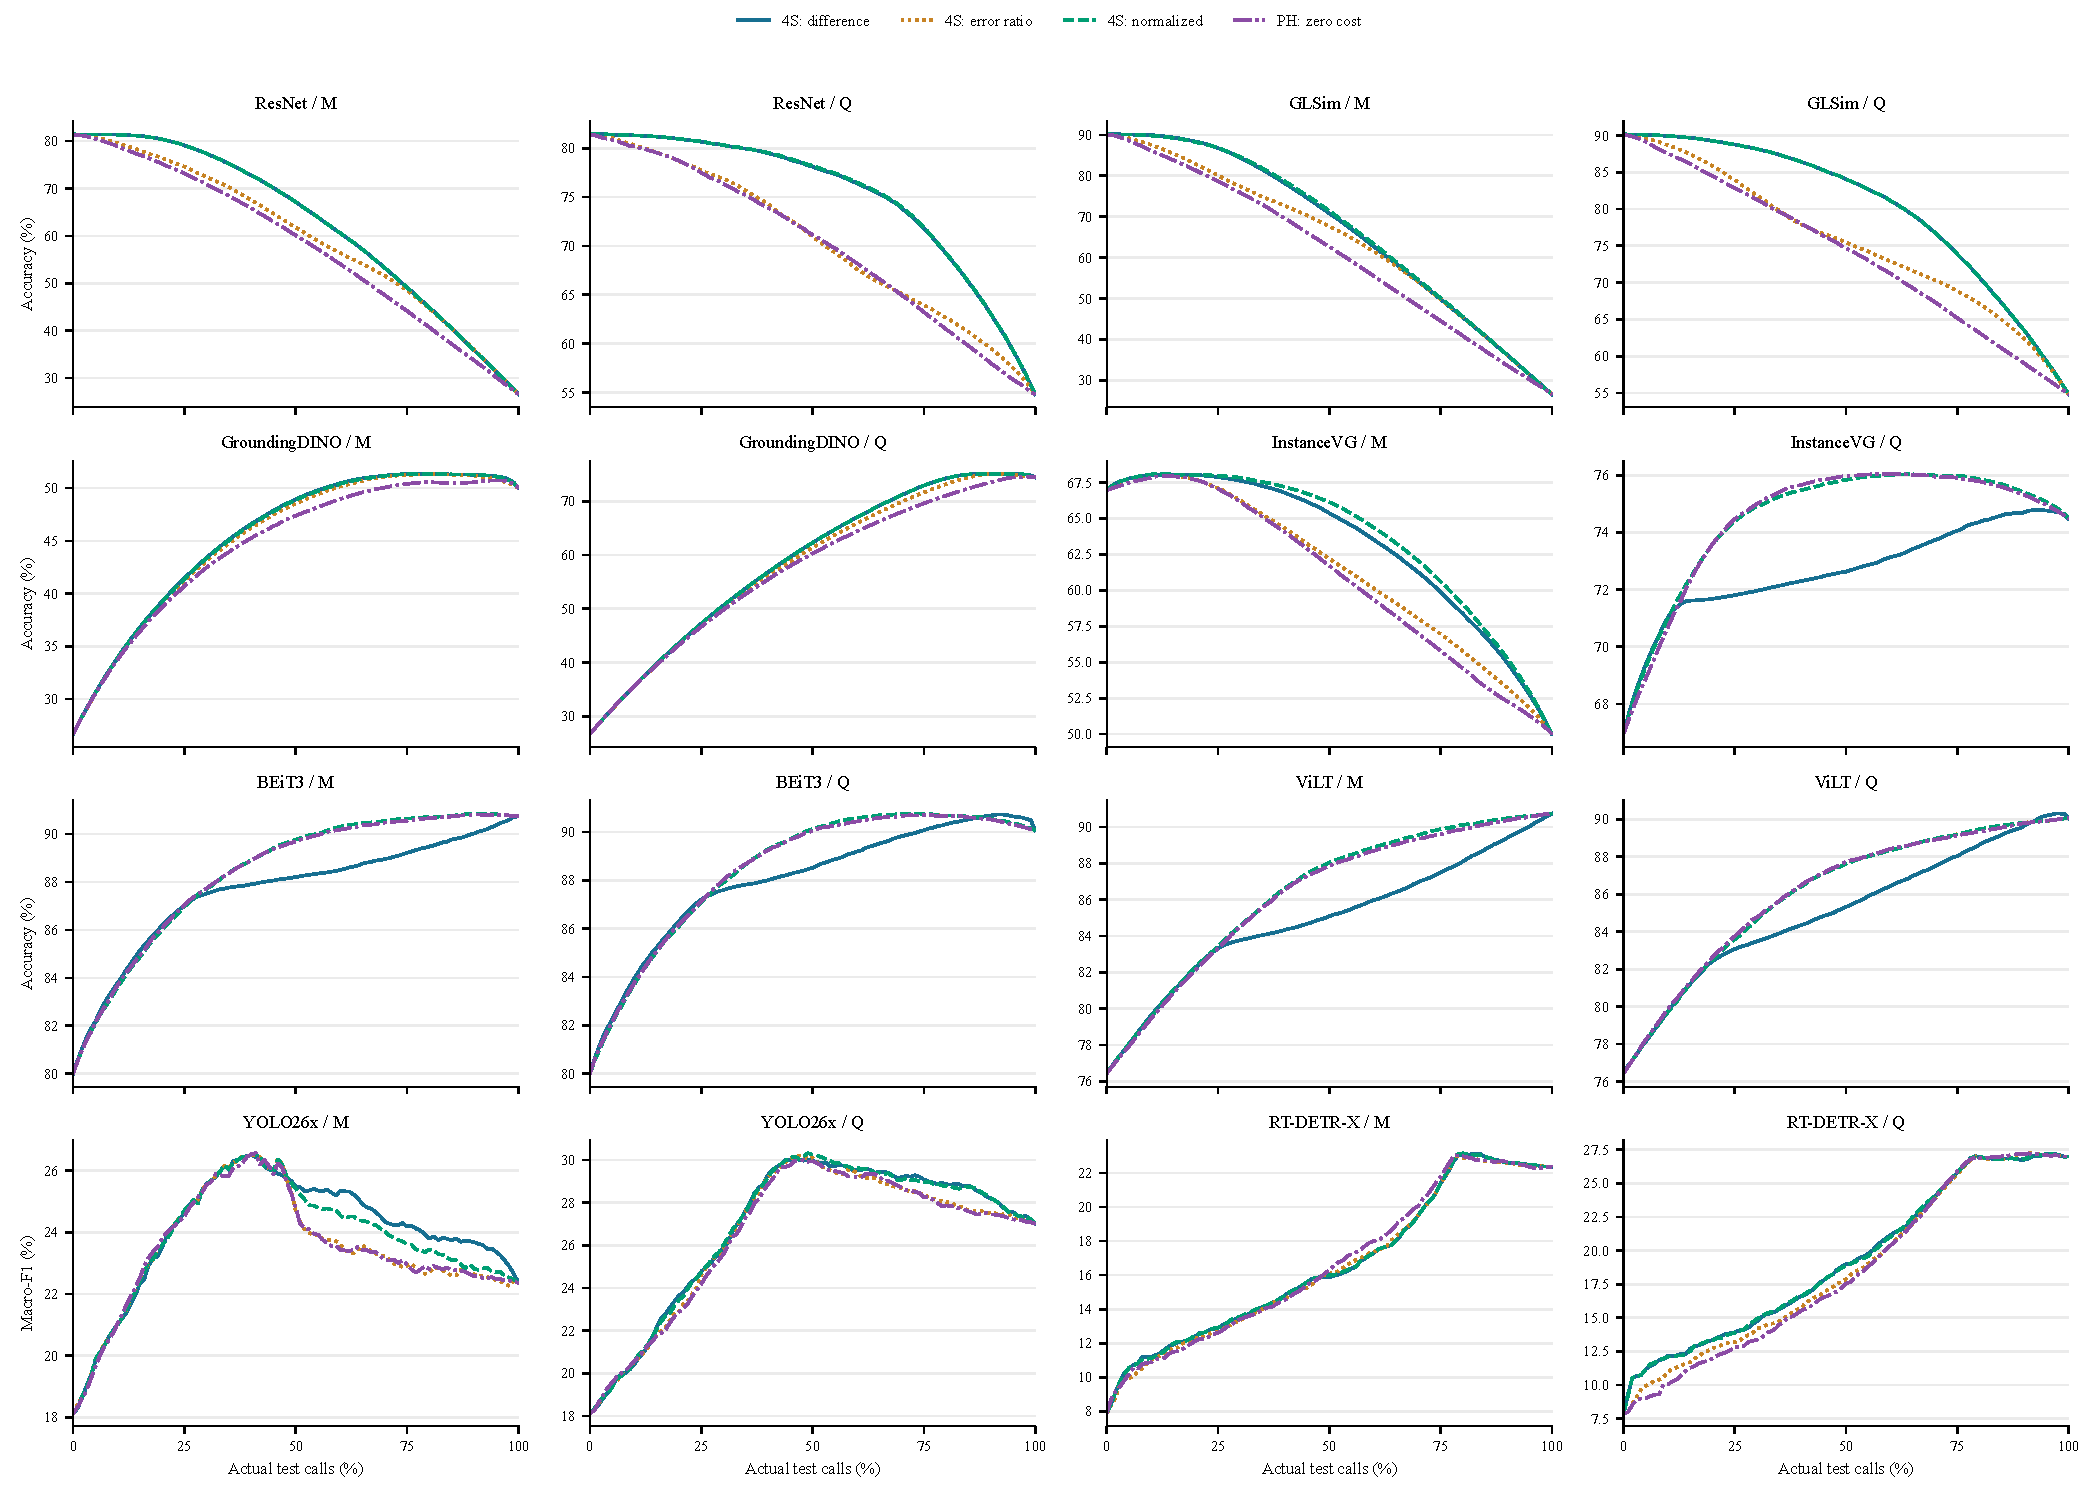
\includegraphics[width=\textwidth]{figures/score_controls.pdf}\caption{Earlier experiments: changing four-state scoring while holding weights fixed, with separately trained zero-cost post-hoc deferral. Both use the archived checkpoint-selection range. These are equal-call curves, not test-selected best-threshold envelopes.}\end{figure}
\clearpage
The full-curve three-state versus four-state differences are below 0.1 points for each task. On NLVR2, changing the same four-state checkpoints from probability difference to error-ratio ranking improves the 25--100\% curve mean from 87.82 to 89.09, close to post-hoc's 89.03. On CUB, the ratios instead reduce performance. This supports a task-dependent scoring effect, not a claim that supervision never matters. The true conditional gain remains optimal for equal costs and additive accuracy; estimated probabilities need not preserve its ideal ranking. Construction macro-F1 is non-additive.

The earlier eighteen-setting architecture search, data-fraction studies and joint-training experiments retain their archived settings; they are not ablations of the final full-budget recipe. They are not used here to claim that each input branch is necessary. Similarly, the older objective table that mixed separately selected ratio checkpoints is superseded by the same-checkpoint scoring comparison above.

\section{Choice of Deferral Baselines}
Post-hoc deferral~\cite{posthocdefer} learns when to replace an existing predictor's answer, which matches the fixed specialist answers used here. Joint classification--deferral methods~\cite{defer,calibrateddefer}, including OvA, instead learn class outputs together with a deferral output. Using their native class branch would change the answer when the VLM is not called; replacing that branch with a fixed specialist would change the original method. Moreover, a single class output does not directly represent a set of grounding boxes or multiple safety-event labels. These methods can be studied on classification subsets or with explicit adaptations, but are not interchangeable baselines for all four tasks under fixed answers. The event-averaged post-hoc loss used for construction is also an adaptation; we do not claim the original classification guarantees for macro-F1.

\section{Cost Estimates}
Figures use measured component costs for the same router architecture: specialist and router costs are paid on every input, with VLM cost added at the actual call rate. Confidence omits the router. Component measurements used 64 inputs at batch size 1 on an A800. These are serial component-based estimates, not newly measured integrated latency; the extra normalization arithmetic was not separately benchmarked. Costs at the selected thresholds have been recomputed from the new call rates.
\clearpage
\subsection{Prompts and Generation Settings}
The following templates come from the paired-prediction collection. Number words for 4 and 16 are displayed as digits here. The original prompt files are retained with the code. Placeholders are replaced by each sample's expression or statement. CUB supplies all 200 candidate classes in a single request; its full class list is supplied with the code. Both VLMs receive the same task input, but their templates may differ. All requests use temperature zero, with limits of 8 tokens for CUB and NLVR2, 512 for gRefCOCO and 768 for ConstructionSite. NLVR2 sends the left image followed by the right image, with these roles explicitly marked. Qwen disables thinking for CUB and NLVR2; MiniCPM constrains these answers to the class index or True/False. Localization and event requests use JSON schemas. Invalid answers are retained and counted as errors without repair or a second model call.

\subsubsection{CUB-200-2011}
\paragraph{MiniCPM-V-4.5}
\VerbatimInput[fontsize=\footnotesize,breaklines=true,breakanywhere=true]{data/reproduction/cub_MiniCPM_prompt.txt}
\paragraph{Qwen3.8-27B-FP8}
\VerbatimInput[fontsize=\footnotesize,breaklines=true,breakanywhere=true]{data/reproduction/cub_Qwen3.8_prompt.txt}

\subsubsection{gRefCOCO}
\paragraph{MiniCPM-V-4.5}
\VerbatimInput[fontsize=\footnotesize,breaklines=true,breakanywhere=true]{data/reproduction/grefcoco_MiniCPM_display.txt}
\paragraph{Qwen3.8-27B-FP8}
\VerbatimInput[fontsize=\footnotesize,breaklines=true,breakanywhere=true]{data/reproduction/grefcoco_Qwen3.8_prompt.txt}

\subsubsection{NLVR2}
\paragraph{MiniCPM-V-4.5}
\VerbatimInput[fontsize=\footnotesize,breaklines=true,breakanywhere=true]{data/reproduction/nlvr2_MiniCPM_prompt.txt}
\paragraph{Qwen3.8-27B-FP8}
\VerbatimInput[fontsize=\footnotesize,breaklines=true,breakanywhere=true]{data/reproduction/nlvr2_Qwen3.8_prompt.txt}

\subsubsection{ConstructionSite}
\paragraph{MiniCPM-V-4.5}
\VerbatimInput[fontsize=\footnotesize,breaklines=true,breakanywhere=true]{data/reproduction/construction_MiniCPM_display.txt}
\paragraph{Qwen3.8-27B-FP8}
\VerbatimInput[fontsize=\footnotesize,breaklines=true,breakanywhere=true]{data/reproduction/construction_Qwen3.8_display.txt}

\clearpage
\subsection{Earlier Prompt Comparisons}
Figures below reproduce earlier prompt comparisons on training subsets: 300 expressions for gRefCOCO and 400 examples each for CUB and NLVR2. Construction uses its recorded training selection. The source label Construction10K refers to ConstructionSite. These curves use the earlier task metrics (including gRefCOCO F1), so their absolute values are not directly comparable with the final routing table. They document prompt choice, not router ablations or new test-time tuning. The experiment ledger retains the input subset and metric for every point.
\begin{figure}[H]\centering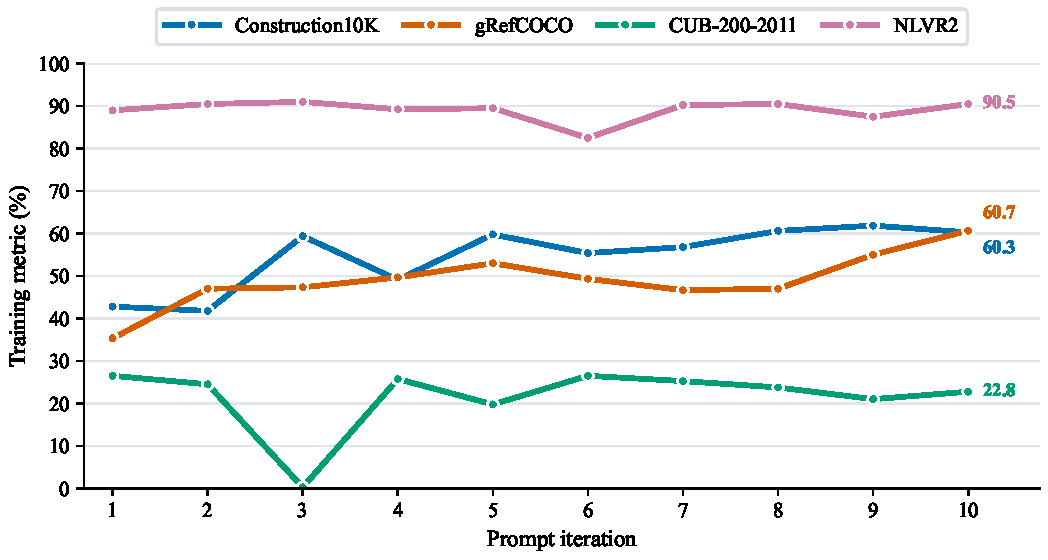
\includegraphics[width=\textwidth]{figures/prompt_iteration_curves_minicpm.pdf}\caption{Earlier MiniCPM prompt comparisons from the recorded experiment ledger.}\end{figure}
\begin{figure}[H]\centering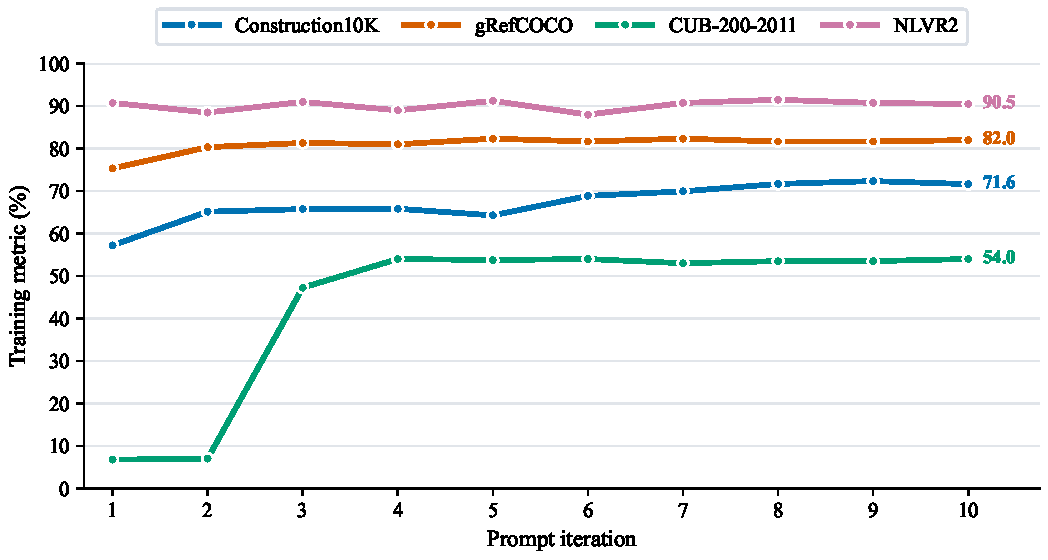
\includegraphics[width=\textwidth]{figures/prompt_iteration_curves_qwen38.pdf}\caption{Earlier Qwen prompt comparisons from the same ledger.}\end{figure}

\bibliographystyle{IEEEbib}
\bibliography{references}
\end{document}
